% Auto-generated figure snippet for PC1 block analysis
\begin{figure}[t]
  \centering
  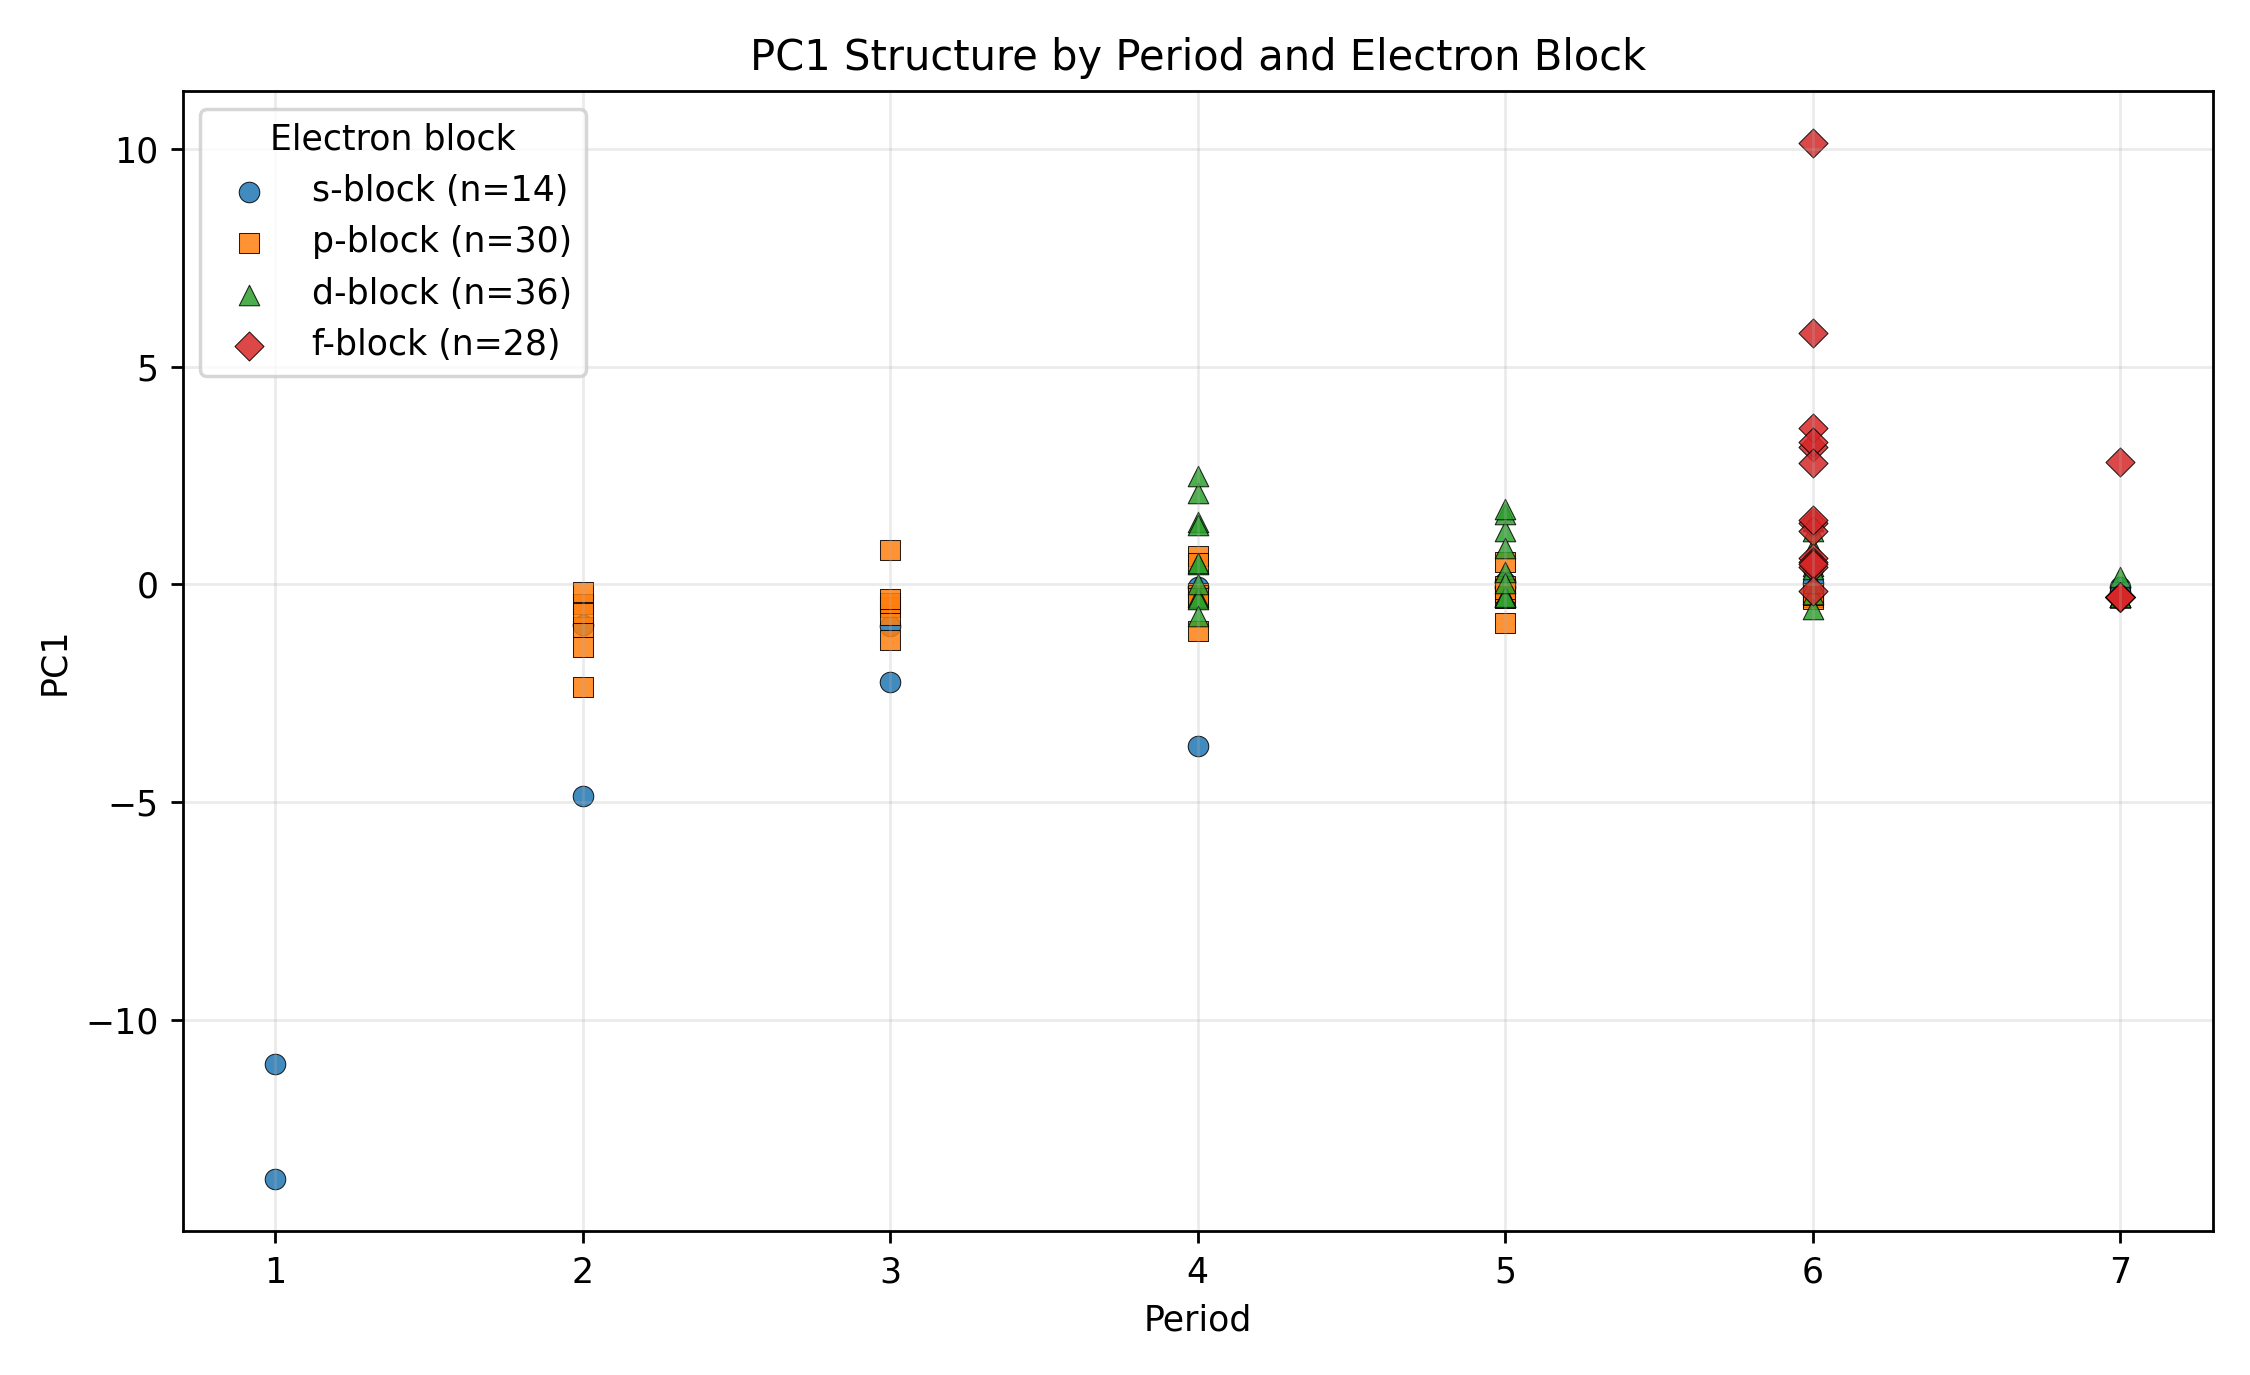
\includegraphics[width=0.85\linewidth]{figures/fig_pc1_vs_period_block.png}
  \caption{PC1 versus period, colored by electron block (s/p/d/f).}
  \label{fig:pc1-period-block}
\end{figure}

\begin{figure}[t]
  \centering
  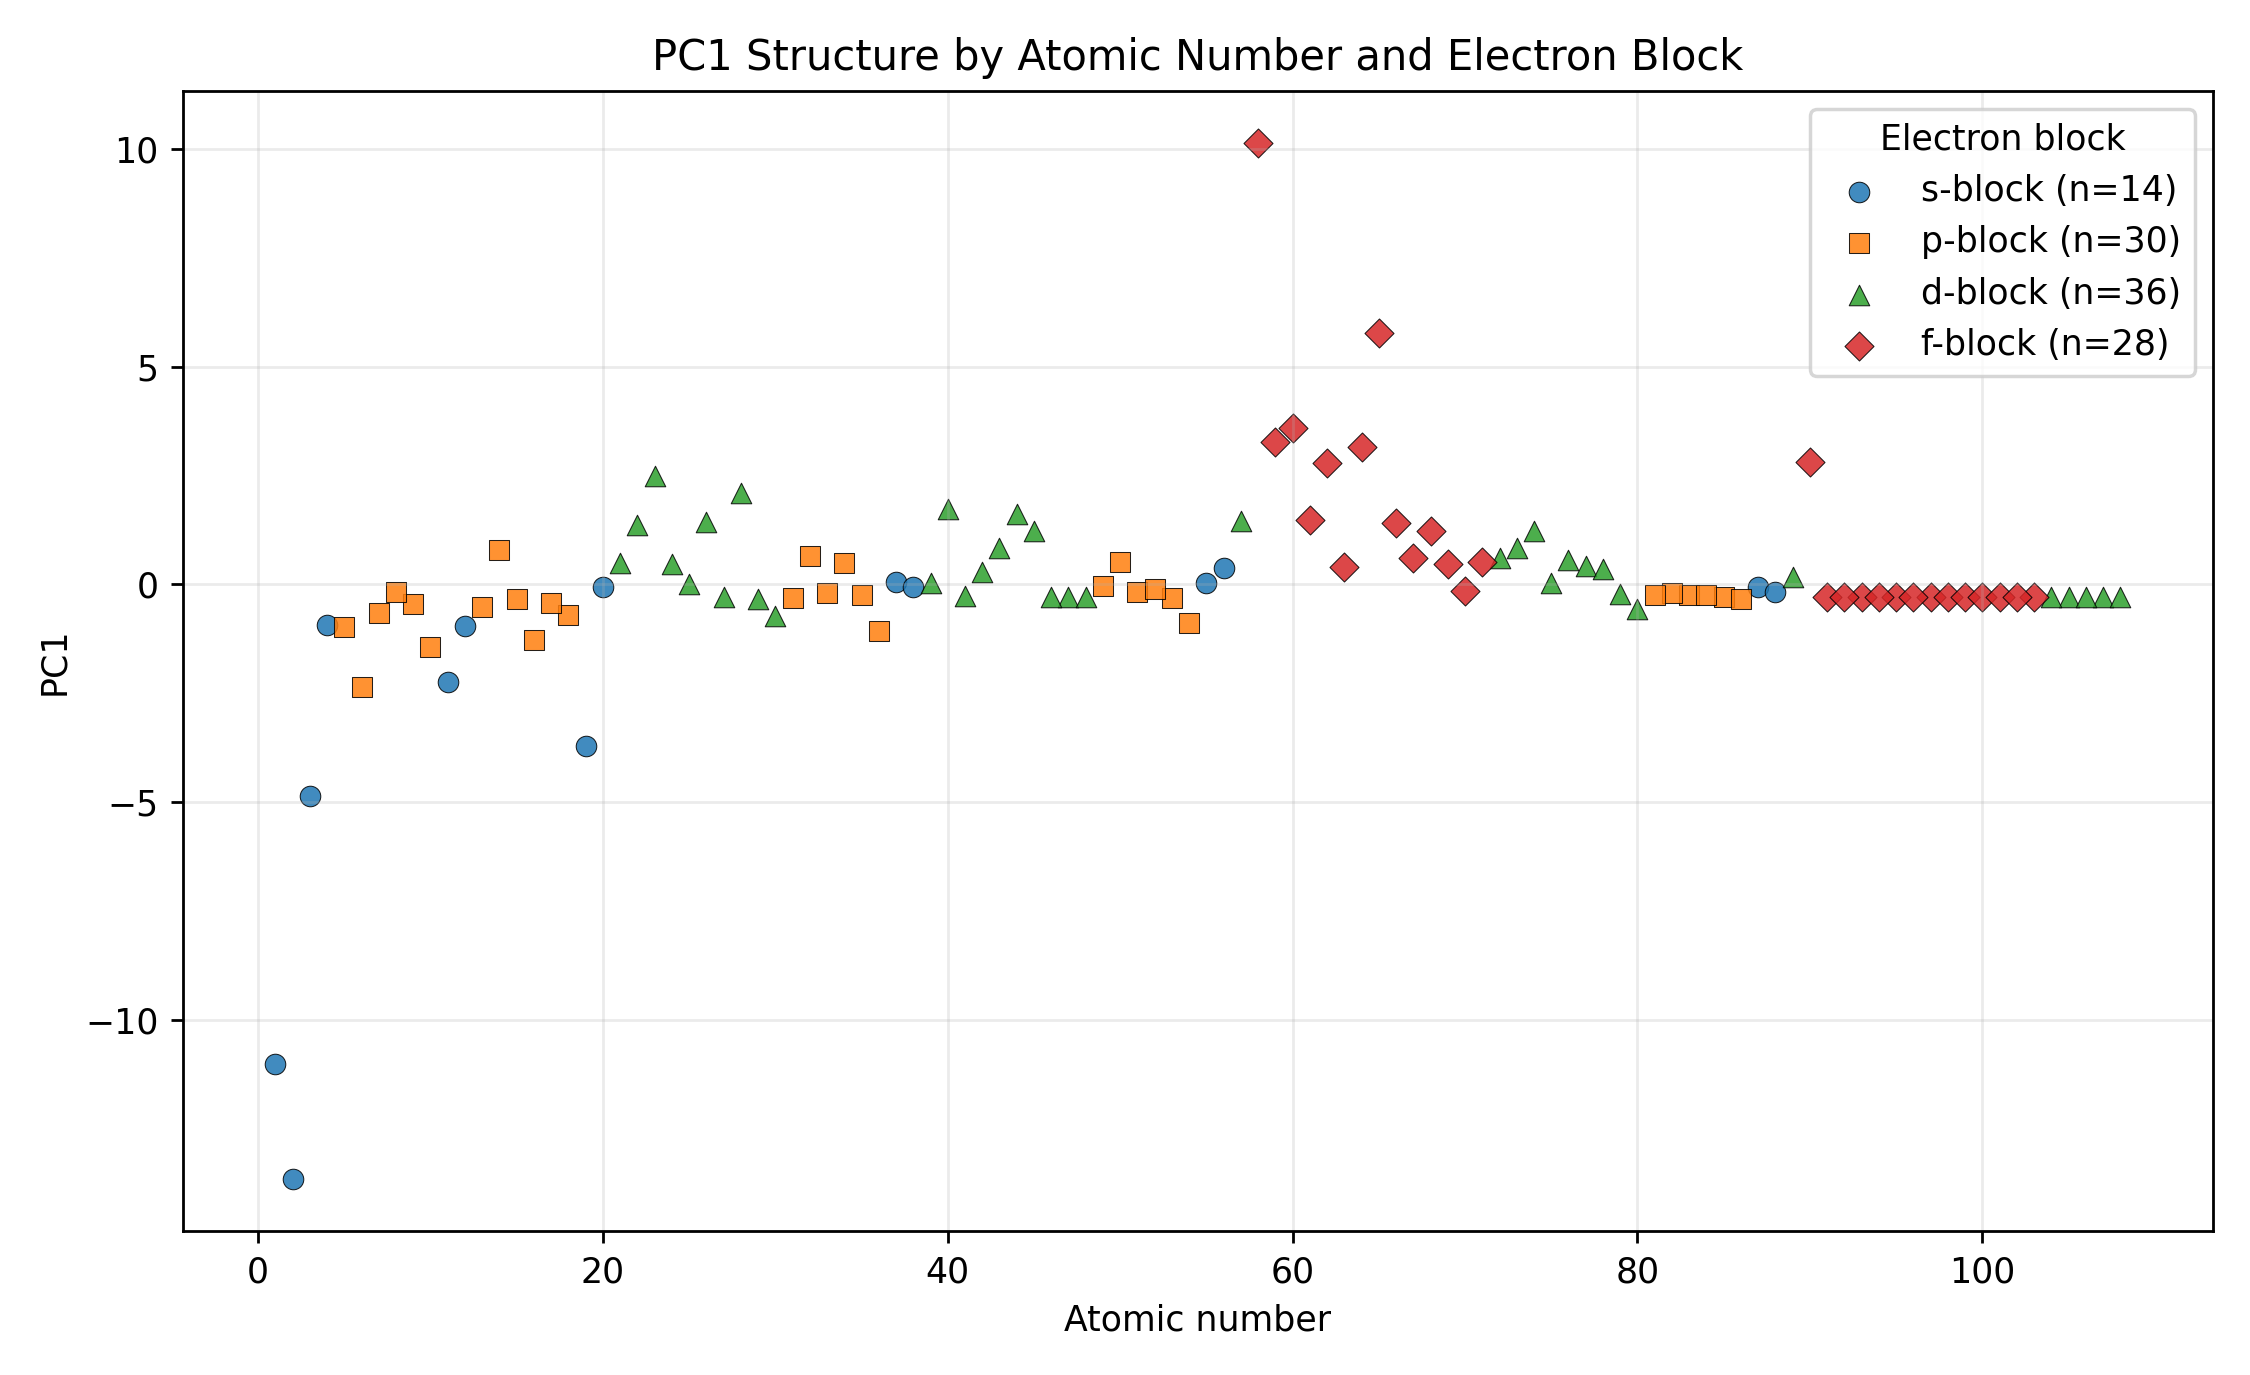
\includegraphics[width=0.85\linewidth]{figures/fig_pc1_vs_atomic_number_block.png}
  \caption{PC1 versus atomic number, colored by electron block (s/p/d/f).}
  \label{fig:pc1-z-block}
\end{figure}

\begin{figure}[t]
  \centering
  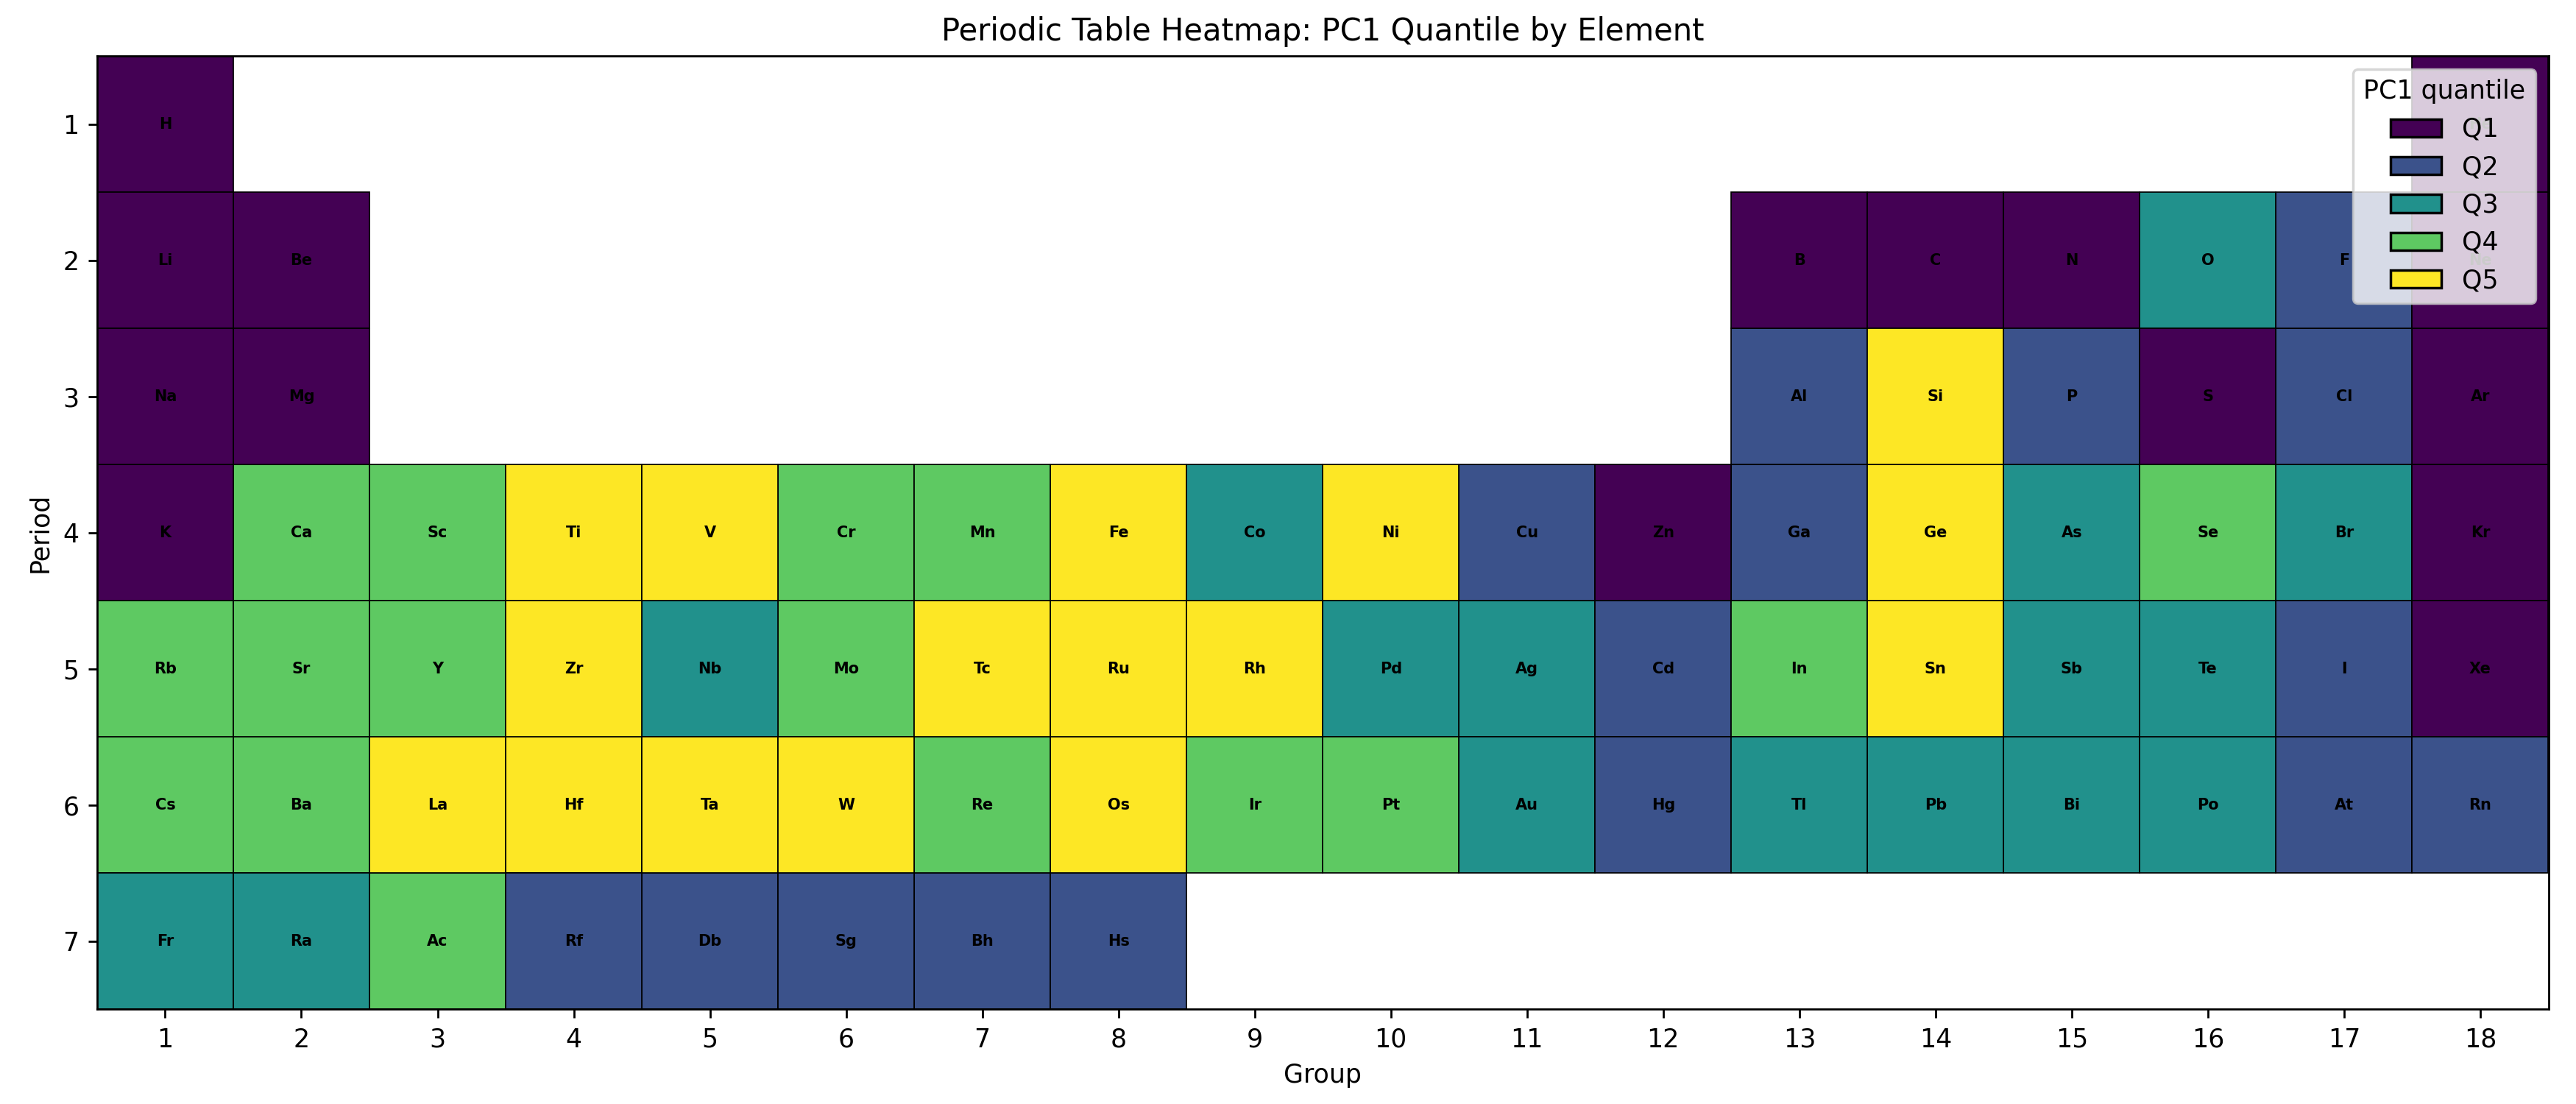
\includegraphics[width=0.95\linewidth]{figures/fig_periodic_table_pc1_heatmap.png}
  \caption{Periodic-table layout with cells colored by PC1 quantile (Q1--Q5).}
  \label{fig:ptable-pc1-heatmap}
\end{figure}

\begin{figure}[t]
  \centering
  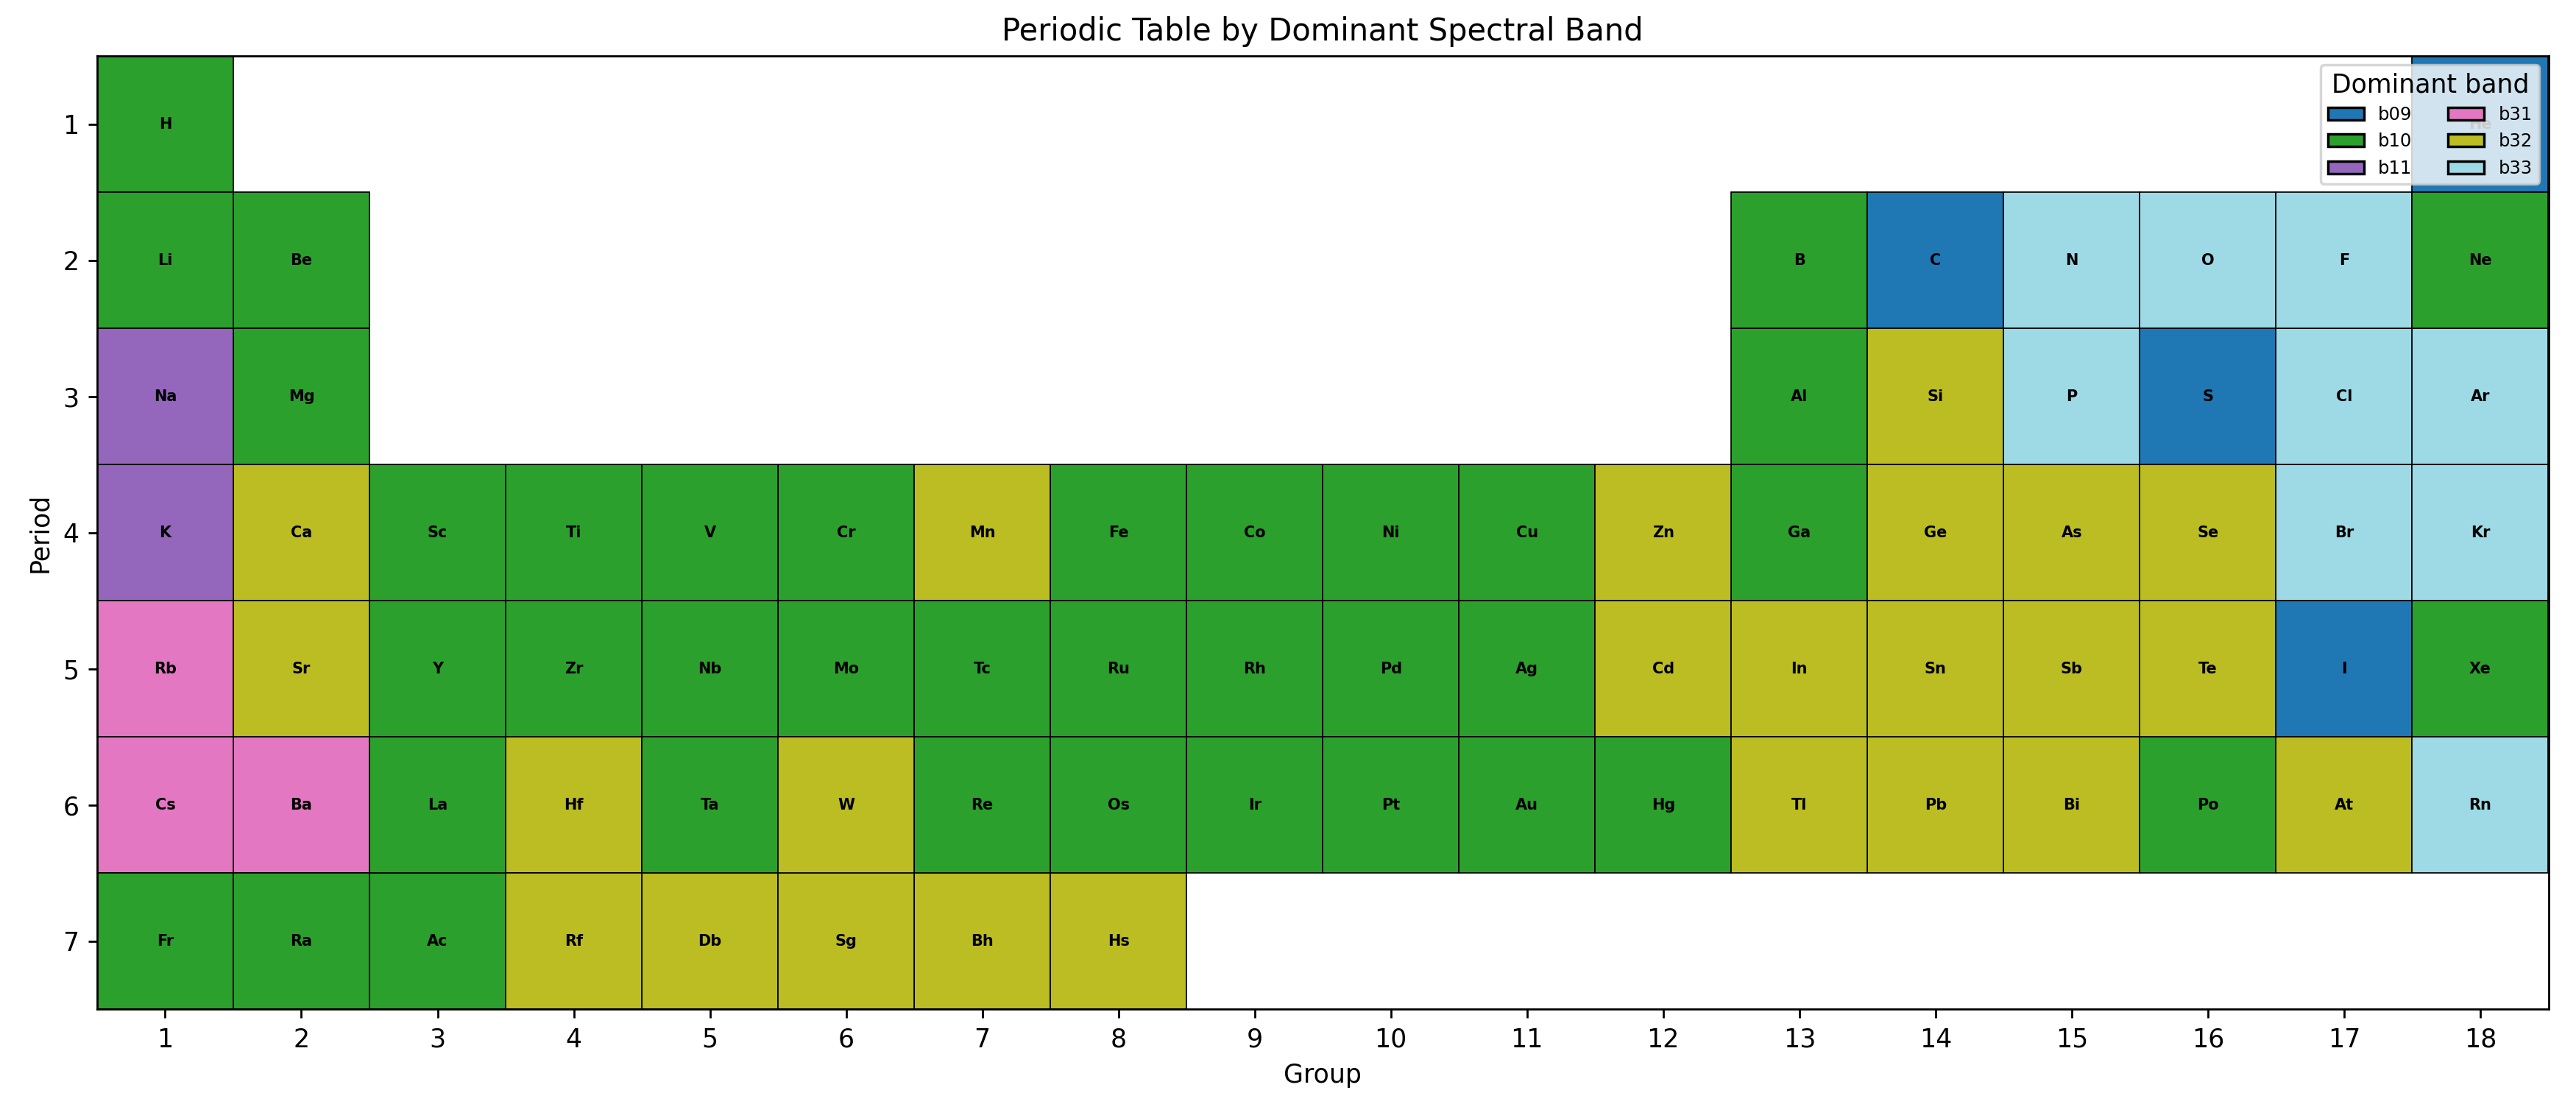
\includegraphics[width=0.95\linewidth]{figures/fig_periodic_table_dominant_band.png}
  \caption{Periodic-table layout colored by dominant spectral band.}
  \label{fig:ptable-dominant-band}
\end{figure}
